\documentclass[11pt,letterpaper]{article}

\usepackage{amsmath}
\usepackage{amssymb}
\usepackage{fancyhdr}
\usepackage{tikz}

\oddsidemargin0cm
\topmargin-2cm
\textwidth16.5cm
\textheight23.5cm

\newcommand{\question}[1] {\vspace{.25in} \hrule\vspace{0.5em}
\noindent{\bf #1} \vspace{0.5em}
\hrule \vspace{.10in}}
\renewcommand{\part}[1] {\vspace{.10in} {\bf (#1)}}

\newcommand{\myname}{Karan Sikka}
\newcommand{\myandrew}{ksikka@cmu.edu}
\newcommand{\myhwnum}{06}

\setlength{\parindent}{0pt}
\setlength{\parskip}{5pt plus 1pt}

\pagestyle{fancyplain}
\lhead{\fancyplain{}{\textbf{HW\myhwnum}}}
\rhead{\fancyplain{}{\myname\\ \myandrew}}
\chead{\fancyplain{}{80-311}}

\begin{document}

\medskip

\thispagestyle{plain}
\begin{center}                  % Center the following lines
{\Large 80-311 Assignment \myhwnum} \\
\myname \\
\myandrew \\
\today
\end{center}

\question{1.1}
$$ \mathtt{THM}(\varphi) \iff (\exists \triangle (\mathtt{PRF}(\triangle, \varphi))) $$

\question{1.2}
Self-reference lemma: \\
If $\varphi(x)$ is any formula in the language of ZF
with exactly the indicated free variable then there is a sentence $\psi$
such that:

$$ ZF \vdash (\psi \iff \varphi('\psi')) $$

Obtaining Godel's sentence G: \\
Let $\psi = G$ and $\varphi = \neg \mathtt{THM}$. Then we substitute into the self reference lemma to obtain:

$$ ZF \vdash (G \iff \neg \mathtt{THM}('G')) $$

\question{1.3}
Assume that ZF is consistent, and assume for sake of contradiction that $ZF \vdash \mathtt{THM}('G') \implies G$.

Then by the defn of G:
$ZF \vdash \mathtt{THM}('G') \implies \neg \mathtt{THM}('G')$.

Which is basically saying for some formula $\varphi$ where $\varphi$ is $G$:
$ZF \vdash \varphi \implies \neg \varphi$.

Which is saying that it's provable in ZF that ZF is inconsistent, and this is contradictory to our assumption that ZF is consistent. Therefore
if ZF is consistent then our assumption that $ZF \vdash \mathtt{THM}('G') \implies G$ is false.

\question{2.1}


\begin{center}
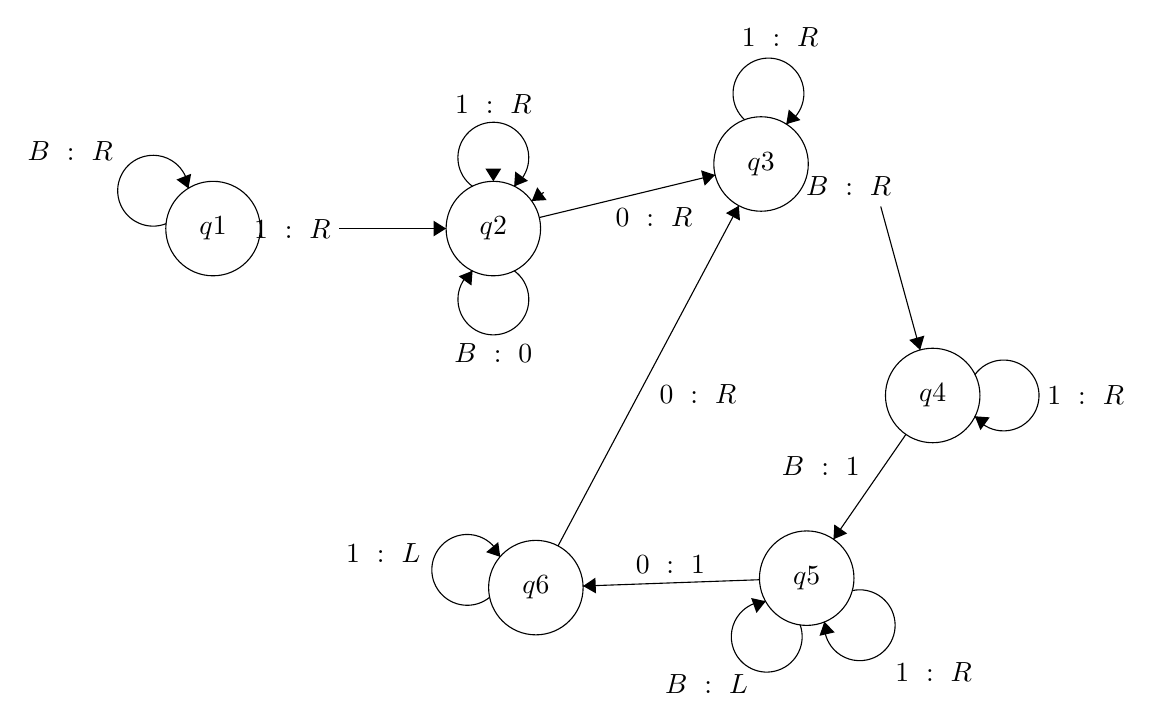
\begin{tikzpicture}[scale=0.2]
\tikzstyle{every node}+=[inner sep=0pt]
\draw [black] (13.9,-21) circle (3);
\draw (13.9,-21) node {$q1$};
\draw [black] (31.7,-21) circle (3);
\draw (31.7,-21) node {$q2$};
\draw [black] (48.7,-16.9) circle (3);
\draw (48.7,-16.9) node {$q3$};
\draw [black] (59.6,-31.6) circle (3);
\draw (59.6,-31.6) node {$q4$};
\draw [black] (51.6,-43.2) circle (3);
\draw (51.6,-43.2) node {$q5$};
\draw [black] (34.4,-43.8) circle (3);
\draw (34.4,-43.8) node {$q6$};
\draw [black] (10.928,-20.687) arc (291.72436:3.72436:2.25);
\draw (7.57,-16.1) node [left] {$B\mbox{ }:\mbox{ }R$};
\fill [black] (12.34,-18.45) -- (12.51,-17.52) -- (11.58,-17.89);
\draw [black] (21.9,-21) -- (28.7,-21);
\draw (21.4,-21) node [left] {$1\mbox{ }:\mbox{ }R$};
\fill [black] (28.7,-21) -- (27.9,-20.5) -- (27.9,-21.5);
\draw [black] (31.7,-18) -- (31.7,-18);
\fill [black] (31.7,-18) -- (32.2,-17.2) -- (31.2,-17.2);
\draw [black] (34.9,-18.7) -- (34.14,-19.25);
\fill [black] (34.14,-19.25) -- (35.08,-19.19) -- (34.49,-18.38);
\draw [black] (30.377,-18.32) arc (234:-54:2.25);
\draw (31.7,-13.75) node [above] {$1\mbox{ }:\mbox{ }R$};
\fill [black] (33.02,-18.32) -- (33.9,-17.97) -- (33.09,-17.38);
\draw [black] (34.62,-20.3) -- (45.78,-17.6);
\fill [black] (45.78,-17.6) -- (44.89,-17.3) -- (45.12,-18.28);
\draw (41.9,-19.63) node [below] {$0\mbox{ }:\mbox{ }R$};
\draw [black] (33.023,-23.68) arc (54:-234:2.25);
\draw (31.7,-28.25) node [below] {$B\mbox{ }:\mbox{ }0$};
\fill [black] (30.38,-23.68) -- (29.5,-24.03) -- (30.31,-24.62);
\draw [black] (47.665,-14.097) arc (227.99099:-60.00901:2.25);
\draw (49.91,-9.48) node [above] {$1\mbox{ }:\mbox{ }R$};
\fill [black] (50.3,-14.37) -- (51.2,-14.11) -- (50.46,-13.44);
\draw [black] (56.3,-19.6) -- (58.8,-28.71);
\draw (54.26,-18.95) node [above] {$B\mbox{ }:\mbox{ }R$};
\fill [black] (58.8,-28.71) -- (59.07,-27.8) -- (58.11,-28.07);
\draw [black] (62.28,-30.277) arc (144:-144:2.25);
\draw (66.85,-31.6) node [right] {$1\mbox{ }:\mbox{ }R$};
\fill [black] (62.28,-32.92) -- (62.63,-33.8) -- (63.22,-32.99);
\draw [black] (57.9,-34.07) -- (53.3,-40.73);
\fill [black] (53.3,-40.73) -- (54.17,-40.36) -- (53.35,-39.79);
\draw (55,-36.05) node [left] {$B\mbox{ }:\mbox{ }1$};
\draw [black] (54.481,-43.992) arc (102.36646:-185.63354:2.25);
\draw (57.19,-49.14) node [right] {$1\mbox{ }:\mbox{ }R$};
\fill [black] (52.72,-45.97) -- (52.41,-46.86) -- (53.38,-46.64);
\draw [black] (51.179,-46.159) arc (19.6409:-268.3591:2.25);
\draw (45.24,-49.27) node [below] {$B\mbox{ }:\mbox{ }L$};
\fill [black] (49,-44.67) -- (48.07,-44.46) -- (48.41,-45.41);
\draw [black] (48.6,-43.3) -- (37.4,-43.7);
\fill [black] (37.4,-43.7) -- (38.22,-44.17) -- (38.18,-43.17);
\draw (42.94,-42.92) node [above] {$0\mbox{ }:\mbox{ }1$};
\draw [black] (31.474,-44.409) arc (309.49413:21.49413:2.25);
\draw (27.1,-41.63) node [left] {$1\mbox{ }:\mbox{ }L$};
\fill [black] (32.14,-41.85) -- (32.01,-40.91) -- (31.24,-41.55);
\draw [black] (35.81,-41.15) -- (47.29,-19.55);
\fill [black] (47.29,-19.55) -- (46.47,-20.02) -- (47.36,-20.49);
\draw (42.23,-31.51) node [right] {$0\mbox{ }:\mbox{ }R$};
\end{tikzpicture}
\end{center}

\question{2.2}





\end{document}

